\documentclass[11pt, twocolumn]{article}

\usepackage{cite}
\usepackage{graphicx}
\usepackage{stfloats}
\usepackage{amsthm}
\usepackage[english]{babel}
\usepackage{authblk}
\usepackage{multicol}
\usepackage{array}
\usepackage[T1]{fontenc}
\usepackage[utf8]{inputenc}
\usepackage{indentfirst}
\usepackage{enumerate}
\usepackage{multirow}
\DeclareGraphicsExtensions{.png}

\title{A Technical Analysis of Developing Hybrid Mobile Applications}
\author[1]{Andrew Zurn\\Computer Science Department\\Saint John's University\\Collegeville, MN\\awzurn@csbsju.edu}

\begin{document}
\maketitle
\begin{abstract}
Mobile application development has been a rapidly evolving area with various platforms, languages and models that are used to build applications for various devices.  In the past, mobile apps have mainly been built on native frameworks, such as Java for Android, or Objective-C for iOS devices, which has caused developers to build multiple native applications, where little to no code has been able to be reused across platforms.  Hybrid mobile applications offer a solution to this, allowing developers to write a common code base and use it across a variety of mobile operating systems.  The focus of this paper will be to explore the issues in mobile development today, and mainly how exactly hybrid development functions to solve these problems.\\
\end{abstract}

\section{Introduction}
\setlength\parindent{.75cm}
Mobile application development is an area within the computing industry that has seen a lot of development and shifts in the past half-decade.  Mobile devices and applications have begun to replace many traditional desktop applications, and had allowed many jobs, activities, and ideas to become portable.  As such, developing for the mobile platform has become an important area of research and development for various industry organizations, and has seen its fair share of popular discoveries and innovations.  Over the course of these past few years, we've seen the technologies used to develop mobile applications go from platform-independent web technologies to OS specific platforms where each device had their own software development kit (SDK). ~\cite{Corral2011}  The shift towards the device dependent SDKs has, however, brought about its own issues, mainly forcing developers to adapt applications to multiple platforms, which can be very costly and time consuming.~\cite{Leroux2011}  However, a new shift has begun, towards creating applications that leverage web technologies, such as HTML5, CSS, and JavaScript, in addition to the platform specific SDKs, to build native-feeling applications.~\cite{Xanthopoulos2013}  This "hybrid" development paradigm, and the general technical details behind it, will be the main focus of this paper, which will also include a comparative discussion of a prototype made both in a native language (Android) and a hybrid counterpart using a platform called {\it Appcelerator}.~\cite{Appcelerator} \\

\section{Background}
Mobile application development had its true beginnings around 2008 with the introduction of the iPhone.  It was at that time that the intention of Apple was to only let developers create mobile web applications for the device.  It wasn't too long after that however, when Google enetered the market and introduced it's mobile solution, Android, onto the market, and with it the Android SDK.  Apple followed Google's leap into the market soon after though with its own SDK for iOS (iPhone's operating system).~\cite{Mims2013} \\

The Android and iOS SDKs, however, are vastly different in their programming models.  Jake Hird, the Director of Research and Education at Econsultancy Australia, in his article, {\it The fight gets technical: mobile apps vs. mobile sites}, provides a brief examination of these two platforms, and a few reasons as to why native development was mainly used to build mobile applications.  He states,

\begin{quote}
Native apps are programmed using Objective C on the iPhone or using Java on Android devices.  Native apps make use of all the phone's features, such as the mobile phone camera, geolocation and the user's address book.   Native apps also do not need to be connected to the internet to be used.  A native app is specific to the mobile handset it is run on, since it uses the features of that specific handset.  Finally, native apps can be distributed on the phone's market place (Apple Store for iPhone (Play Store for Google)). ~\cite{Hird2011}
\end{quote}

The syntactical differences between Java and Objective-C can be seen in Figures 1 and 2 below.\\

\begin{figure}[h]
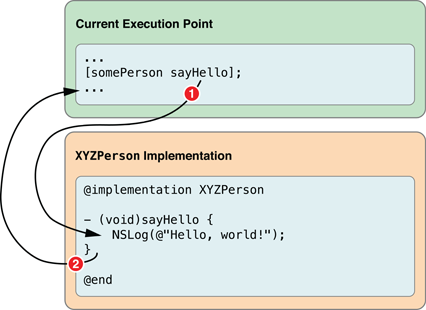
\includegraphics[scale=0.5]{objectiveChelloWorld}
\caption{Objective-C Hello World program ~\cite{Developer.Apple.com}}
\end{figure}

\begin{figure}[h!]
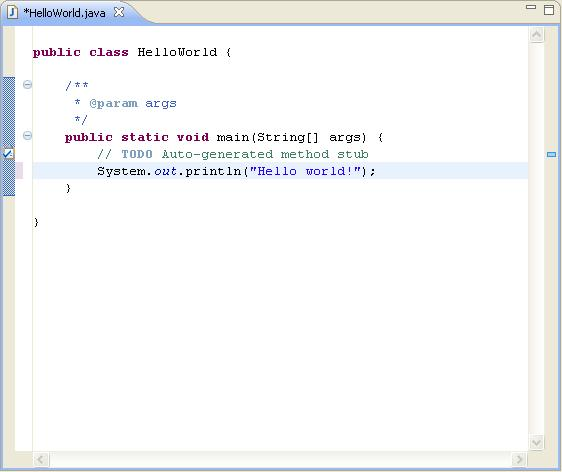
\includegraphics[scale=0.5]{java-hello-world}
\caption{Java Hello World program ~\cite{Made-Easy.com}}
\end{figure}

As can be seen, Objective-C and Java are rather different languages, and even further, the frameworks and developing tools around them differ even more.  As such, building the same application natively for both platforms can become rather complex and require different skill sets.  Spyros Xanthopoulos, in his article, {\it A Comparative Analysis of Cross-platform Development Approaches for Mobile Applications}, highlights the "major disadvantage" of developing different native applications, that being that "it is not possible to reuse the source code for another platform; (thus) the very same app must be redeveloped from scratch."~\cite{Xanthopoulos2013}  To further our problem, we can look to the words of Olivier Le Goaer and Sacha Waltham, researchers of the mobile app development, who summarize both the current state of the development landscape, and the problems that characterize it.

\begin{quote}
We have definitively entered an era of mobility.  Evidence of that is the phenomenal growth of mobile markets, in terms of both the numbers of devices sold and number of downloaded mobile applications.  But this growth has been accompanied by a fragmentation of the mobile platform, which seriously complicates the task of mobile apps developers.  An application must be made available on as many platforms as possible in order to reach diverse user bases... Every platform comes with its own SDK and requires specific programming skills, in terms of both languages and API.  As such, this heterogeneity creates very important additional redevelopment costs for software developers, who are thus compelled to focus their skills on just a few platforms, usually only two or three.  It is worth mentioning that this lack of sustainability in software development was already encountered in the past, and therefore Model-Driven Architecture returns centre-stage with the slogan: "{\it Write Once, run everywhere}".~\cite{Goaer2013}
\end{quote} 

Because of the problems native development has caused, we are now beginning to see a new shift today towards the aforementioned 'hybrid' approach, where mobile applications are being developed to be compatible across the large variety of devices on the market. ~\cite{Kolokolov2013} \\

\section{Technical Analysis}
Hybrid application development, although relatively new, has various working implementations that don't all adhere to one set model of development.  In this section, a more generalized analysis of the area as a whole will be presented, along with a more detailed analysis of the platform {\it Appcelerator}, which is just one platform of many that present a functional hybrid solution.

\subsection{Languages and Platforms}
In their article, Goaer and Waltham provide a great look at the various platforms that have become the top competitors in building hybrid applications, of which a few are worth noting.  The first is {\it Apache Cordovo}.\\

\begin{quote}
{\it Apache Cordova} (www.phonegap.com) operates by interpreting HTML5/CSS3 code for views, and JavaScript code using an abstraction API, allowing system and hardware access.  The user interface is presented like a "chromeless web browser, used as a WebView (calls UIWebView in iOS, class Webview in Android.  Packaged binaries include the browser and the application sources. ~\cite{Goaer2013}
\end{quote}

This approach effectively builds a common application that would be more or less run from a phone's internet browser, with its dynamic features coming from JavaScript that also has device feature access.  The app is run in a web-view, which allows for an application that can be downloaded onto any device, and would run like a web application.  The next platform they look at is {\it Appcelerator Titanium}.\\

\begin{quote}
{\it Titanium} (www.appcelerator.com) precompiles JavaScript code into a set of symbols, resolved based on the targeted mobile OS (compiled .o files for iOS, .class files for Android).  When resolution is over, and the generated dependency matrix can be understood by the front-end, the adequate back-end compiler is called to compile it into binaries  Those also include a JavaScript interpretor, packages with the application for performance reason, and reading dynamic code. ~\cite{Goaer2013}
\end{quote}

Essentially, the JavaScript that is generated into these 'symbols' are the functions that each device will call on when a natively build component (buttons, textboxes, etc.) is interacted with by the user. ~\cite{Heitkoetter2013}\\

Another approach that has been essentially developed for creating hybrid mobile applications is the use of a 'Domain Specific Language' (DSL). Goaer states that a DSL effectively "captures sufficiently common and high-level concepts to be shared by different platforms.  This DSL then outputs native code."  One such example of this type of hybrid approach is {\it APPlause}, which "generates native iOS, Android, or Windows Phone 7 code.  That code, Java, Objective-C, C\#, or Python, is human-readable, and can be reworked before deployment." ~\cite{Goaer2013} \\

One final platform they look at is the CodenameOne project, which translates Java code to another platform-specific language.

\begin{quote}
CodenameOne is a Java-based platform, allowing to create real native apps, on several mobile platforms. Using plugsin for NetBeans or Eclipse, a developer can build an application using Java and a Swing-like API, and a drag-and-drop GUI builder.  Apps are then deployed, directly in Java for Android, BlackBerry, and JavaME devices; for iOS the code is translate to C/Objective-C using XMLVM (a translation tool); for Windows Phone a C\# translator is used. ~\cite{Goaer2013}
\end{quote}

Figure 3 presents a comparison of all the major entities that have a hybrid mobile platform solution, and offers some insight into how they achieve cross-platform compatibility, and how well they compare against native applications.\\

\begin{figure*}
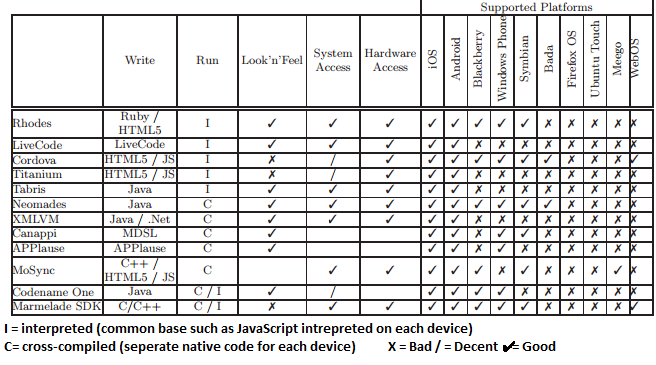
\includegraphics[width=\textwidth, height=8cm]{cross-platform-chart}
\caption{Comparison of Hybrid Development Platforms ~\cite{Goaer2013}}
\end{figure*}

Overall, what hybrid application development breaks down to is how you want to develop your applications.  One approach is to build a mobile web application, and wrap it inside of a "thin native container where access to device features can be done through specialized APIs," such as JavaScript libraries. ~\cite{Xanthopoulos2013}  The next option would be to develop on a platform such as {\it Appcelerator}, which also builsd applications out of a common base of web technologies, but will natively build the UI components and link the dynamic aspects of the application to those components. ~\cite{Xanthopoulos2013}  The final option is to build your application in an environment, such as CodenameOne, or using a DSL that will cross-compile the code into the respective frameworks to be deployed on the wide variety of devices.  In the end, each have their advantages over native design.  Building your application out of hybrid technologies tends to be easier than having to acquire the knowledge to build applications out of native frameworks, and overall, each of these solutions provide an option to obtain the goal of "write once, run everywhere." ~\cite{Goaer2013}

\subsection{Performance}
One of the larger areas of discussion in the hybrid mobile application development is how hybrid application performance stacks up against natively developed applications.  In their article, {\it Evaluation of mobile app paradigms}, Ngu Phuc Huy and Do vanThanh evaluate the various development options for building mobile applications, and give a brief examination of the underlying performance of hybrid applications against native applications.  Their work was mainly done using the {\it PhoneGap} platform, and compared against a similar application that was build natively.  In their article they state,

\begin{quote}
Native apps are well-known for their fast and responsive user interface, and the seamless capability to access hardware features... PhoneGap uses the same native APIs with native apps but abstracts them so that developers can simply write apps in HTML and Javascript... However PhoneGap apps cannot replace native apps because they perform slower than native apps due to the overhead from abstraction and HTML rendering in addition to the time to execute the native processes. ~\cite{Huy2012}
\end{quote}

Brian Leroux and Andre Charland, in their article, {\it Mobile Application Development: Web vs. Native}, solidifies Huy's and vanThanh's statements, exclaiming "execution time is, of course, a key facet of performance.  When interpreting code (as we do for the Web with JavaScript), the more there is to interpret, the longer the execution time.  Here the Web technology stack has some catching up to do.  JavaScript, for all its leaps in performance, is still slower than native counterparts." ~\cite{Leroux2011}\\

Huy and vanThahn are able to quantify this, by showing the amount of time in milliseconds a user takes to interact with their separately built applications.  As can be seen in Figure 4, their native application took the least amount of time on average to be used, the hybrid application build in {\it PhoneGap} took the second longest to use, and the HTML5 application took the longest on average to use.

\begin{figure}[h]
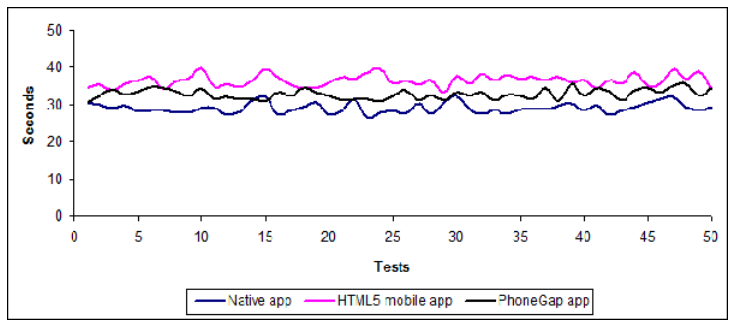
\includegraphics[scale=0.4]{huy-app-performance}
\caption{The amount of time to use the native app, HTML5 mobile app and PhoneGap app in comparison ~\cite{Huy2012}}
\end{figure}

Overall, hybrid applications haven't come to perform as fast as native applications yet. As the JavaScript interpreter performance increases however, we might one day see these hybrid applications perform just as fast as their native counterparts, which will be a huge benefit in making them an even more viable replacement for natively built apps than they are today.

\subsection{Hybrid compared to Native Development}
Another area within the mobile development debate, is how developing hybrid applications compares to developing native applications.  One of the obvious driving factors in building hybrid applications is that it massively reduces the amount of time needed to develop, as a single code base is used to port to the various target platforms.  As Luis Corral explains in his article, {\it Evolution of Mobile Software Development from Platform-Specific to Web-Base Multiplatform Paradigm}, "conducting the whole development process for a single application for each platform will eventually become redundant, expensive, and unpractical."  By adopting these new hybrid technologies, as he states, "it will allow developers to structure a software process for a variety of platforms, targeting their final products to a wider extent of potential customers by conducting a single development process only." ~\cite{Corral2011}\\

\begin{figure*}
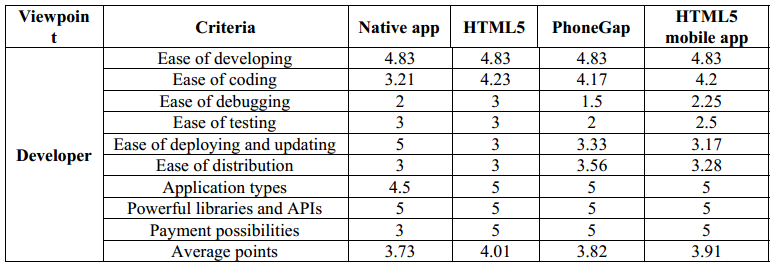
\includegraphics[width=\textwidth, height=4.5cm]{hybrid-native-compare-table}
\caption{Comparison of Native, HTML5, and Hybrid Development ~\cite{Huy2012}}
\end{figure*}

This argument can again be supported with data from Huy's and vanThahn's research, where they were able to survey and score how well developing in the hybrid environment {\it PhoneGap} did compared to both its HTML5 and native counterpart.  As can be seen in Figure 5, the ease of developing the hybrid application was on par with the native app, but coding the app was actually easier when done in the hybrid platform.  The overall score of the PhoneGap app is also better than the native app, which shows that hybrid mobile app development is just as easy, if not more so, than developing an application in a native language.  In the end, Huy's and vanThahn's work underscores how developing hybrid applications is becoming an effective replacement for native apps, as developing and coding a hybrid application proves to be a much easier task.\\


\section{Discussion}
In order to further evaluate the technical aspects of hybrid development, two prototypes applications were built, one natively in Android, and the other built using the hybrid platform {\it Appcelerator Titanium}.~\cite{Appcelerator}.\\

\subsection{Application Information}

The objective of the prototype, at this time called 'HIPAA Security Training,' was to build a training/reference course for those in the medical field to use to obtain their HIPPA Security and Privacy Administration certification, which is required to be updated annually.  The app presents a very rudimentary course by presenting the user with a list of chapters, then a list of sections within each chapter, and finally a detail page that contains reading material.  Although this application is merely a prototype, it does highlight some of the key differences in building applications in a native language and the {\it Appcerelator Titanium} development environment.

\subsection{How Appcelerator Works}

{\it Appcelerator Titanium} is actually an all-in-one integrated development environment (IDE) that deploys a hybrid application.  The environment builds interpreted hybrid applications, where the UI objects of an application are build natively using each platforms SDK, and the dynamic features of the application are written in a common language, that is JavaScript. ~\cite{Xanthopoulos2013}\\

The JavaScript used within the application is understood in each platform is presented in the research of Olivier Goaer. {\it Appcelerator} compiles the JavaScript into "a set of symbols," that will be able to be interpreted by each of the mobile operating systems.  Those symbols will be in ".o files for iOS, and .class file for Android."  Essentially, it will create the compiled code that implements the functions written in JavaScript (which means that effectively it cross-compiles the JavaScript code to Java, Objective-C, or another language, depending on the target platform.)~\cite{Goaer2013}  Tim Poulsen, the Director of Training and Curriculum Development at Appcelerator, Inc. provides additional insight into the inner functions of this development environment.  The {\it Appcelerator Titanium} platform uses each targeted device's SDK, and along with the Titanium SDK, builds native applications that can be pushed out to the device's app store.  Ultimately, the multiple device SDKs will be used to build the native components, a developer will write in JavaScript, and the Titanium SDK will compile that JavaScript into the necessary program files that will be packaged with the native components.  Figure 6 offers a visual of how the development environment does this.~\cite{Poulsen2012}

\begin{figure}[h]
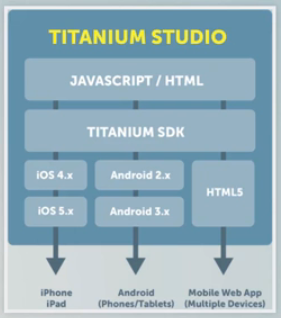
\includegraphics[scale=1]{appcelerator-flow-chart}
\caption{Flow Chart on how {\it Appcelerator} Builds Native Applications ~\cite{Poulsen2012}}
\end{figure}

\subsection{Developing with Android}
The process of developing the native Android app proved tedious and difficult more so than it did not.  The application was originally build using a Master/Detail template provided by the eclipse development environment.  The application uses Java to load an XML View object, that then loads a Fragment object (an object that can be added or removed from the View dynamically though the app lifecycle), of which finally contains a list container that loads in the chapter content for the course.  The chapter content is stored in as a TreeMap object within a .txt file and is read in via a ObjectReader.  From  there, when a user selects a chapter, the Java then has to load a new fragment, with a new list container that contains all the section data for that chapter.  Finally, when a section is selected, a new TextView is created, where the section text is loaded into the view to be read by the user.\\

What made the development of this Android application rather frustrating was the over complexity of having to use several different objects, all in order to display a simple list on the screen.  Rather than being able to simply display a list containing all the data in the initial view, the ListContainer object being used mandated it be put into a Fragment, which would then have to be loaded into a View object.  From there, the app had to keep track of what chapter the user selected, or rather, what row in the list they selected, and pass it back to the original View object.  Then, the View object would pass the chapter parameter to a new View, and that View would then have to go through the whole process again in order to display a list of sections for that chapter.  Overall, the Android application made for a rather messy implementation of the training course application through it's necessity to take encapsulation to an overbearing extreme.\\

\subsection{Developing with Appcelerator Titanium}
The process of re-building the application on the {\it Appcelerator Titanium} platform, although there was some difficulty in doing the initial setup of the IDE, was a lot smoother and easier to implement than it's Android counterpart had been.  In this application a Master/Detail template was again used as a starting point to develop the course layout.  The layout of this application is similar to the Android app, as a initial View object was loaded onto the screen which contained the rows of selectable chapters.  From there, each chapter would open a new View that would have the chapter's section in it.  Finally, the section would open a final View that would have the reading material on the page.\\

The inner workings of the hybrid app are a little less complicated than it's Android relative, and made for a much faster development time.  The application is initially launched by a JavaScript module, of which would create all the global properties that the other modules within the application would need to know about to call upon.  It would also load all of the needed views immediately as to create as little processing time between actions in the app as necessary.  From here, the application opens the first View object, which simply creates a table of rows and attaches it to it's View object.  A listener also within this module is used to wait for the user to select a row in the table, of which then would pass that row number to the next View.  That View would then pull from the section data for that chapter from an internal array, and build a table out of that data, which is then again attached to it's View.  Finally, another listener would wait for a row to be selected, which would open a final View object, which contains the text for that specific section.  Overall, the ability to more easily create lists to be displayed in this hybrid app made for a much more expedient development time.\\

\subsection{Comparing the Counterparts}
The development of these two applications, as briefly discussed above, proved vastly different, not only in the technologies and techniques they used, but also in the difficulty and amount of time needed in developing each application.  The {\it Appcelerator} application took the majority of half a day to understand, design and implement, due to it's natural way of only delegating tasks when it is needed.  Conversely, developing the native application for this course made for more than a few difficulties, and took a good portion of a week in order to implement.  Rather than simplifying the development process, multiple modules that shared very like functionality had to be created, and a complex messaging system between those modules had to be implemented in order to maintain a stable lifecycle between all the View objects that would be presented on the screen.  Overall, as was earlier summarized by Huy and vanThanh in there similar experiment of developing a application using different platform, the ease of coding this application was won over by the {\it Appcelerator} platform, which made developing this application multitudes easier than developing it's native counterpart.\\

When looking at the actual resources of the two applications, the {\it Appcelerator} built hybrid application obviously shows its distinctiveness by having a fraction of the code needed to develop the Android application.  The overall lines of code (LOC) in the Android application, between both Java and XML files, is along the lines of 1000.  The LOC within the {\it Appcelerator} application is right at 410.  The amount of classes and XML files in the Android project was 18, while the hybrid counterpart was 6 JavaScript files.  The single screen of these working prototypes  can be seen in Figures 7 and 8 below.

\begin{figure}[h!]
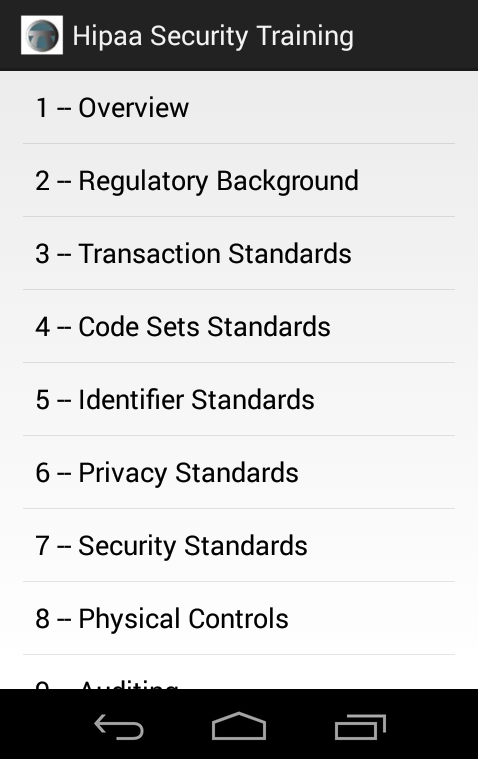
\includegraphics[scale=0.35]{android-chapter-implementation}
\caption{The Android implementation showing a list of Chapters within the course.}
\end{figure}

\begin{figure}[h!]
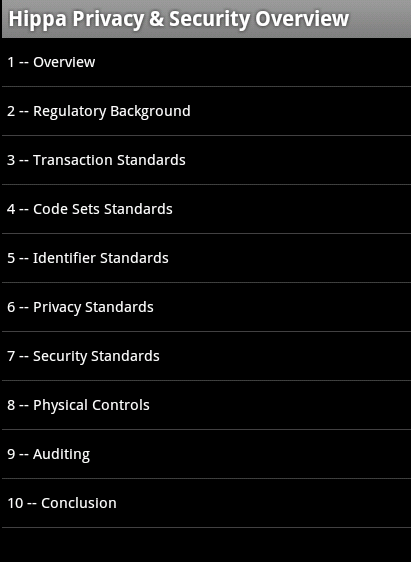
\includegraphics[scale=0.4]{appcelerator-chapter-implementation}
\caption{The Hybrid implementation showing a list of Chapters within the course.}
\end{figure}

Additionally, two code examples are displayed below, both of which do essentially the same function within the application, that is, display the first View which shows a list of Chapters.  As one might notice, the code found in the {\it Appcelerator} figure is quite straightforward to read, and no real comments are needed to describe the logic of the program.  When we look at the Android code however, one will see an excess amount of variables needed to hold the state of the applications, a variety of interfaces and extending classes, and methods and syntax that is hard to read and understand.

\begin{figure}[h!]
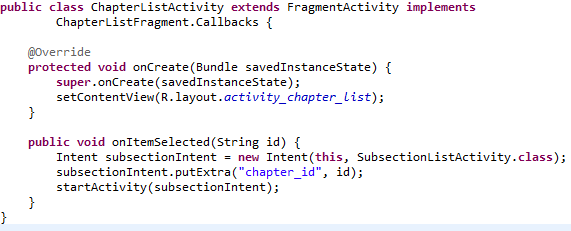
\includegraphics[scale=0.62]{android-chapter-list-code}
\caption{The Android native code used to hold the chapter list.}
\end{figure}

\begin{figure}[h!]
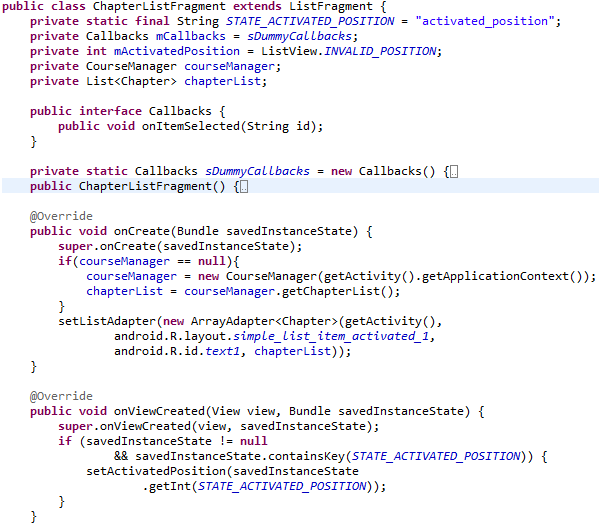
\includegraphics[scale=0.5]{android-chapter-fragment-code}
\caption{A portion of the Android native code used to produce the Chapter fragment that holds the ListContainer object.}
\end{figure}

\begin{figure}[h]
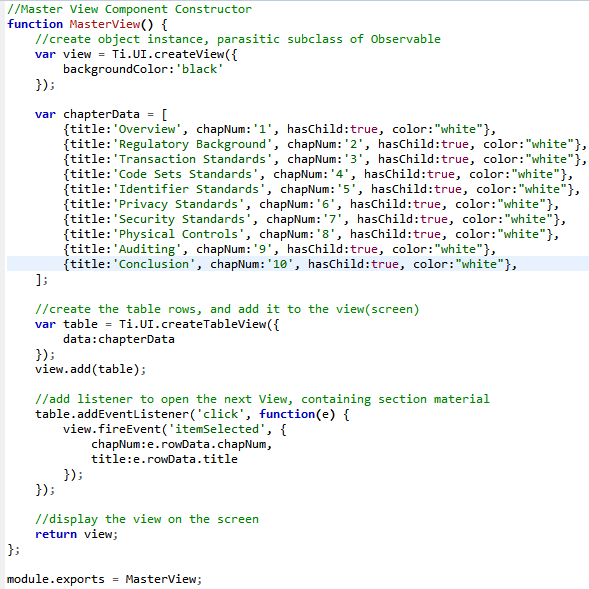
\includegraphics[scale=0.62]{appcelerator-chapter-code}
\caption{The {\it Appcelerator} JavaScript code used to produce the Chapter list inside the application.}
\end{figure}

As can be seen by both implementing an Android application, and then a hybrid counterpart to it, using {\it Appcelerator} proved to be a lot more straight forward in developing, and turned out to be about half the amount of code to produce the same functioning application.  {\it Appcelerator} proved to generate the same functionality, and greatly reduced the cost of developing over an Android application and having to deal with the complexities that are inherent to the Android platform.

\section{Conclusion}
Hybrid application development has become rich in its varying technical implementations and approaches.  Many platforms offer either a way for code such as JavaScript to be interpreted by a mobile device, or even for a common code base to be cross-compiled into the various native languages. {\it Appcelerator}, being in the interpretive camp, provides a way for developers to build a common code base out of JavaScript and HTML, which is used as the dynamic aspect of a mobile application, and the UI features of the app are built using each of the varying devices SDKs, and then linked to those dynamic portions of JavaScript code.  Using these platforms, mobile apps can begin to be built to act much like their native counterparts, and in doing so, actually take much less time, overall code, and knowledge of the various mobile frameworks to develop.  In sum, hybrid application development environment, though relatively new and unheard of, offer very real solutions for developers that want to build their applications to run on the large market of devices currently seen in the mobile world, and might soon replace the traditional native development paradigms.

\bibliographystyle{plain}
\bibliography{TechAnalysisBibs}
\end{document}